\documentclass[11pt,a4paper]{article}

\usepackage[utf8]{inputenc}
\usepackage[T1]{fontenc}
\usepackage[spanish,es-tabla]{babel}
\usepackage[a4paper,top=2.5cm,bottom=2.3cm,left=2.2cm,right=2.2cm,headheight=28pt]{geometry}
\usepackage{array}
\usepackage{tabularx}
\usepackage{booktabs}
\usepackage{colortbl}
\usepackage{xcolor}
\usepackage{enumitem}
\usepackage{fancyhdr}
\usepackage{lastpage}
\usepackage[most]{tcolorbox}
\usepackage{csquotes}
\usepackage[backend=biber,style=ieee]{biblatex}
\usepackage[hidelinks]{hyperref}

\addbibresource{referencias.bib}

\definecolor{uteqgreen}{HTML}{0B7A3B}
\definecolor{uteqdark}{HTML}{075C2C}
\definecolor{midblue}{HTML}{1F5C8B}
\definecolor{rowgray}{HTML}{F2F4F3}
\definecolor{boxbg}{HTML}{F7F9F8}

\newcolumntype{Y}{>{\raggedright\arraybackslash}X}
\newcommand{\thdr}[1]{\cellcolor{uteqgreen}\textcolor{white}{\textbf{#1}}}

\pagestyle{fancy}
\fancyhf{}
\lhead{\footnotesize UTEQ $\cdot$ Ingenier\'ia de Requerimientos (ISR-401) $\cdot$ SPA 2026--2027}
\rhead{\footnotesize TA-PFC-E1 -- Entrega 1}
\lfoot{\footnotesize Sistema de Gesti\'on para Restaurante con IA -- Anaranjoa-UX (Quevedo)}
\rfoot{\footnotesize P\'agina \thepage\ de \pageref{LastPage}}
\renewcommand{\headrulewidth}{0.5pt}
\renewcommand{\footrulewidth}{0.4pt}

\setlength{\parindent}{0pt}
\setlength{\parskip}{5pt}
\renewcommand{\arraystretch}{1.2}

\begin{document}

\begin{titlepage}
    \centering
    \vspace*{0.6cm}
    {\Large\textbf{\textcolor{uteqdark}{UNIVERSIDAD T\'ECNICA ESTATAL DE QUEVEDO}}}\\[0.25cm]
    {\large Facultad de Ciencias de la Computaci\'on}\\[0.15cm]
    {\large Carrera de Ingenier\'ia de Software}\\[0.8cm]

    \textcolor{uteqgreen}{\rule{\linewidth}{1.5pt}}\\[0.5cm]
    {\LARGE\textbf{TA-PFC-E1 -- ENTREGA 1}}\\[0.3cm]
    {\Large Visi\'on, alcance, partes interesadas, contexto y plan de elicitaci\'on}\\[0.45cm]
    \textcolor{uteqgreen}{\rule{\linewidth}{1.0pt}}\\[0.8cm]

    \begin{tcolorbox}[colback=boxbg,colframe=uteqgreen,boxrule=0.8pt,arc=2mm,title={\textbf{Proyecto Fin de Curso}}]
        \centering
        \textbf{Sistema de Gesti\'on para Restaurante con M\'odulo de Inteligencia Artificial}\\
        \textbf{Organizaci\'on cliente: Restaurante Anaranjoa-UX, Quevedo, Los R\'ios}
    \end{tcolorbox}

    \vspace{0.7cm}

    \noindent\begin{tabularx}{\linewidth}{|p{0.30\linewidth}|Y|}
        \hline
        \thdr{Campo} & \thdr{Detalle}\\
        \hline
        Asignatura & Ingenier\'ia de Requerimientos (ISR-401) --- 4.\textsuperscript{o} Nivel, Paralelo B\\
        \hline
        \rowcolor{rowgray} Docente & Gleiston Cicer\'on Guerrero Ulloa, PhD (\texttt{gguerrero@uteq.edu.ec})\\
        \hline
        Unidad & Unidad 2. Elicitaci\'on y An\'alisis de Requisitos\\
        \hline
        \rowcolor{rowgray} Per\'iodo acad\'emico & Segundo Per\'iodo Acad\'emico Ordinario (SPA) 2026--2027\\
        \hline
        Semana y cierre & Semana 4 (16 al 22 de noviembre de 2026) --- Cierre: s\'abado 21 de noviembre de 2026, 23:59\\
        \hline
        \rowcolor{rowgray} Equipo &
        Robinson Espinoza Jeanpierre (L\'ider; visi\'on, alcance y gesti\'on)\\
        & Naranjo Alfonzo Anthony Alexander (Elicitaci\'on y modelado)\\
        & S\'anchez Centeno Roselyn Andreina (An\'alisis y calidad documental)\\
        \hline
        Repositorio & \url{https://github.com/Roselyn15/ISR-401-NRS} (Paralelo B)\\
        \hline
    \end{tabularx}

    \vfill
    {\normalsize Quevedo, Los R\'ios, Ecuador}\\
    {\normalsize Noviembre de 2026}
\end{titlepage}
% La portada no incrementa el contador de pagina; se ajusta para que el pie
% coincida con el total fisico de paginas del PDF.
\addtocounter{page}{1}

\tableofcontents
\newpage

% ==============================================================================
% SECCION 1: FICHA Y ALCANCE (Lider: Robinson Espinoza Jeanpierre)
% ==============================================================================
\section{Ficha del proyecto}

\subsection{Nombre del sistema y organizaci\'on cliente}
El sistema a desarrollar se denomina \textbf{Sistema de Gesti\'on para Restaurante con M\'odulo de Inteligencia Artificial} (en adelante, \emph{SGR-IA}). La organizaci\'on cliente es el \textbf{El Balcón Restaurant}, ubicado en la ciudad de Quevedo, provincia de Los R\'ios, Ecuador. El proyecto se desarrolla en el marco de la asignatura Ingenier\'ia de Requerimientos (ISR-401) del programa Ingenier\'ia de Software de la Universidad T\'ecnica Estatal de Quevedo.

\subsection{Problema u oportunidad}
La operaci\'on de un restaurante concentra en un mismo turno la atenci\'on en sala, el registro de pedidos, la preparaci\'on en cocina, el control de insumos, la facturaci\'on y la atenci\'on de pedidos a domicilio. Cuando estos procesos se apoyan en registros manuales y en comunicaci\'on verbal, aparecen demoras en horas pico, susceptibilidad a errores en la transcripci\'on de pedidos y dificultad para consultar el estado real del inventario. La norma ISO/IEC/IEEE 29148:2018 exige identificar a las partes interesadas y establecer el l\'imite del sistema antes de definir requisitos \cite{iso29148}; en consecuencia, esta entrega se limita a acordar la visi\'on, el alcance, el contexto y la planificaci\'on de la elicitaci\'on, sin adelantar soluciones tecnol\'ogicas. La identificaci\'on de partes interesadas y la delimitaci\'on del contexto se tratan en los fundamentos de ingenier\'ia de requisitos \cite{pohl2025}, mientras que la selecci\'on de t\'ecnicas seg\'un la fuente y el tipo de conocimiento se sustenta en el syllabus IREB \cite{ireb2026}.

\emph{Estado de validaci\'on:} el enunciado del problema se formul\'o a partir del dominio de negocio y ser\'a confirmado, corregido o descartado con el responsable de El Balcón Restaurant durante la primera sesi\'on de elicitaci\'on. Ninguna cifra operativa se presenta como dato medido de la organizaci\'on hasta contar con evidencia registrada.

\subsection{Objetivo general}
Caracterizar la operaci\'on real del El Balcón Restaurant y delimitar un sistema de gesti\'on asistido por inteligencia artificial que integre pedidos, cocina, inventario y ventas, con supervisi\'on humana sobre las decisiones cr\'iticas, como base para la especificaci\'on de requisitos de las entregas posteriores del PFC.

\subsection{Objetivos de negocio medibles}
Los siguientes objetivos son metas acordadas para la elicita\'cion y el dise\~no; sus l\'ineas base se obtendr\'an de la observaci\'on y de los registros de la organizaci\'on:

\begin{enumerate}[leftmargin=18pt,itemsep=4pt]
    \item \textbf{Reducir el tiempo de registro de un pedido.} Obtener una reducci\'on de al menos 30\% del tiempo medio de registro respecto de la l\'inea base medida en la sesi\'on de observaci\'on, con el mismo n\'umero de personas en turno.
    \item \textbf{Disminuir los errores de transcripci\'on de pedidos.} Alcanzar una tasa de errores por pedido igual o inferior a 2\% en una muestra de al menos 50 pedidos posteriores a la puesta en marcha del prototipo.
    \item \textbf{Disponer de informaci\'on de inventario actualizada.} Lograr que el 100\% de los insumos cr\'iticos tenga registro de entrada y salida en el sistema, con al menos una actualizaci\'on por turno y una conciliaci\'on semanal contra el conteo f\'isico.
    \item \textbf{Mejorar la trazabilidad de ventas.} Generar un resumen diario de ventas y productos m\'as solicitados sin transcripci\'on manual adicional, disponible para el responsable antes del cierre de caja.
\end{enumerate}

\section{Alcance del sistema}

\subsection{Dentro del alcance}
\begin{itemize}[leftmargin=18pt,itemsep=2pt]
    \item Registro y seguimiento de pedidos de sala y de entrega a domicilio, con estados visibles para sala y cocina.
    \item Gesti\'on de reservas y de solicitudes especiales de los clientes, con registro de la informaci\'on relevante para cocina.
    \item Control de inventario de insumos, entradas, salidas, alertas de reposici\'on y conciliaci\'on semanal.
    \item Registro de compras y de proveedores, con soporte para la comparaci\'on de precios.
    \item Registro de ventas, medios de pago y generaci\'on de res\'umenes diarios y semanales.
    \item M\'odulo de inteligencia artificial para sugerencias de reposici\'on y de productos complementarios, con explicaci\'on de cada sugerencia y confirmaci\'on humana obligatoria.
    \item Gesti\'on de usuarios por rol y respaldo de la informaci\'on operativa.
\end{itemize}

\subsection{Fuera del alcance}
\begin{itemize}[leftmargin=18pt,itemsep=2pt]
    \item Desarrollo de una aplicaci\'on m\'ovil propia para clientes o de un marketplace de delivery externo.
    \item Integraci\'on con pasarelas de pago, bancos o con el sistema de facturaci\'on electr\'onica del SRI.
    \item Automatizaci\'on de la preparaci\'on de alimentos o sustituci\'on del criterio del personal de cocina en decisiones de higiene, alergias o seguridad alimentaria.
    \item Migraci\'on de informaci\'on hist\'orica anterior al inicio del proyecto.
    \item Capacitaci\'on presencial extensiva y soporte t\'ecnico posterior a la entrega acad\'emica.
\end{itemize}

\section{Restricciones principales}
\begin{itemize}[leftmargin=18pt,itemsep=2pt]
    \item \textbf{Restricci\'on legal y \'etica:} el tratamiento de datos del personal y de los clientes se rige por la Ley Org\'anica de Protecci\'on de Datos Personales del Ecuador \cite{lopdp2021} y por el C\'odigo de \'Etica de la ACM \cite{acm2018}. No se publican datos personales, grabaciones ni documentos firmados en el repositorio p\'ublico.
    \item \textbf{Restricci\'on de supervisi\'on:} las recomendaciones del m\'odulo de inteligencia artificial son orientativas; la decisi\'on final permanece en una persona responsable.
    \item \textbf{Restricci\'on econ\'omica y tecnol\'ogica:} el prototipo se desarrolla con recursos acad\'emicos, sin licencias de pago y con dependencia de la conectividad disponible en el local.
    \item \textbf{Restricci\'on de tiempo:} el cronograma de la asignatura finaliza en la semana 17 del SPA 2026--2027; la gesti\'on del trabajo se organiza seg\'un los principios del PMBOK \cite{pmbok2021}.
    \item \textbf{Restricci\'on de Alcance:} la entrega 1 no incluye requisitos detallados ni dise\~no de soluci\'on; esos productos se derivan de la elicitaci\'on planificada en la secci\'on~3.
\end{itemize}

\section{Declaraci\'on de uso de inteligencia artificial}
Se utiliz\'o asistencia de inteligencia artificial como apoyo para la revisi\'on de redacci\'on y la verificaci\'on de la compilaci\'on \LaTeX{}. Herramienta: asistente integrado del entorno OpenCode y revisor autom\'atico independiente; versi\'on: sesi\'on de 19 de noviembre de 2026. Prop\'osito: detectar incoherencias formales y comprobar que el documento regenera el PDF con \texttt{pdflatex}, \texttt{biber} y dos pasadas adicionales de \texttt{pdflatex}. Verificaci\'on: cotejo manual de cada afirmaci\'on contra las fuentes citadas y ejecuci\'on local del procedimiento de compilaci\'on descrito en el archivo \texttt{README.md}. El contenido t\'ecnico y las decisiones de alcance son de autor\'ia del equipo.


% ==============================================================================
% SECCION 2: PARTES INTERESADAS (Sanchez Centeno Roselyn Andreina) -- commit del 19/11
% ==============================================================================
\section{Partes interesadas}
\sloppy

\subsection{Identificaci\'on y caracterizaci\'on}
Se identifican las partes interesadas como Roles, no como personas, seg\'un lo exigido por ISO/IEC/IEEE 29148:2018 \cite{iso29148} y los fundamentos de ingenier\'ia de requisitos \cite{pohl2025}. La tabla~\ref{tab:stakeholders} registra diez roles, su inter\'es, su influencia, su disponibilidad estimada y la estrategia de participaci\'on propuesta. Los c\'odigos sustituyen a los nombres para evitar la publicaci\'on de datos personales, conforme a la LOPDP \cite{lopdp2021}. La disponibilidad es una estimaci\'on de planificaci\'on, no un dato confirmado por la organizaci\'on.

\begin{table}[htbp]
\centering
\footnotesize
\begin{tabularx}{\linewidth}{|l|p{1.9cm}|Y|p{1.8cm}|p{2.4cm}|X|}
\hline
\thdr{C\'odigo} & \thdr{Rol} & \thdr{Inter\'es principal} & \thdr{Influencia} & \thdr{Disponibilidad} & \thdr{Estrategia de participaci\'on}\\
\hline
AD-01 & Propietario / administrador & Viabilidad econ\'omica y control de la operaci\'on & Alta & Baja & Entrevista individual y validaci\'on final; res\'umenes breves por correo institucional.\\
\hline
GO-01 & Gerente de operaciones & Flujos de sala y cocina sin interrupciones & Alta & Media & Taller de modelado de flujos y revisi\'on de prioridades.\\
\hline
COC-01 & Jefe de cocina & Ordenes claras y tiempos de preparaci\'on & Media & Media & Observaci\'on en turno y entrevista corta posterior.\\
\hline
COC-02 & Personal de cocina & Evitar reprocesos y confusiones & Baja & Media & Observaci\'on an\'onima y preguntas abiertas en el taller.\\
\hline
MES-01 & Mesero/a & Registrar pedidos con rapidez & Baja & Alta & Observaci\'on en sala y cuestionario breve.\\
\hline
CAJ-01 & Cajero/a & Cierre de caja exacto y res\'umenes claros & Media & Media & Entrevista focalizada sobre reglas de cierre.\\
\hline
INV-01 & Encargado de inventario & Existencias suficientes y trazabilidad & Media & Media & Cuestionario estandarizado y revisi\'on de entradas y salidas.\\
\hline
DEL-01 & Repartidor/a & Conocer el estado de cada entrega & Baja & Media & Cuestionario breve de tres preguntas.\\
\hline
CLI-01 & Cliente final & Servicio oportuno y pedido correcto & Baja & Baja & Cuestionario an\'onimo sin datos de identificaci\'on.\\
\hline
PRO-01 & Proveedor local & Reposiciones oportunas & Baja & Alta & Contacto indirecto por medio de INV-01; solo si el responsable lo autoriza.\\
\hline
\end{tabularx}
\caption{Partes interesadas, intereses y estrategia de participaci\'on.}
\label{tab:stakeholders}
\end{table}

\subsection{Matriz poder--inter\'es}
La figura~\ref{fig:matriz} sit\'ua los roles seg\'un su poder de decisi\'on y su inter\'es en el proyecto. La ubicaci\'on es una propuesta derivada de la caracterizaci\'on anterior y se revisar\'a con AD-01 en la sesi\'on de validaci\'on.

\begin{figure}[htbp]
\centering
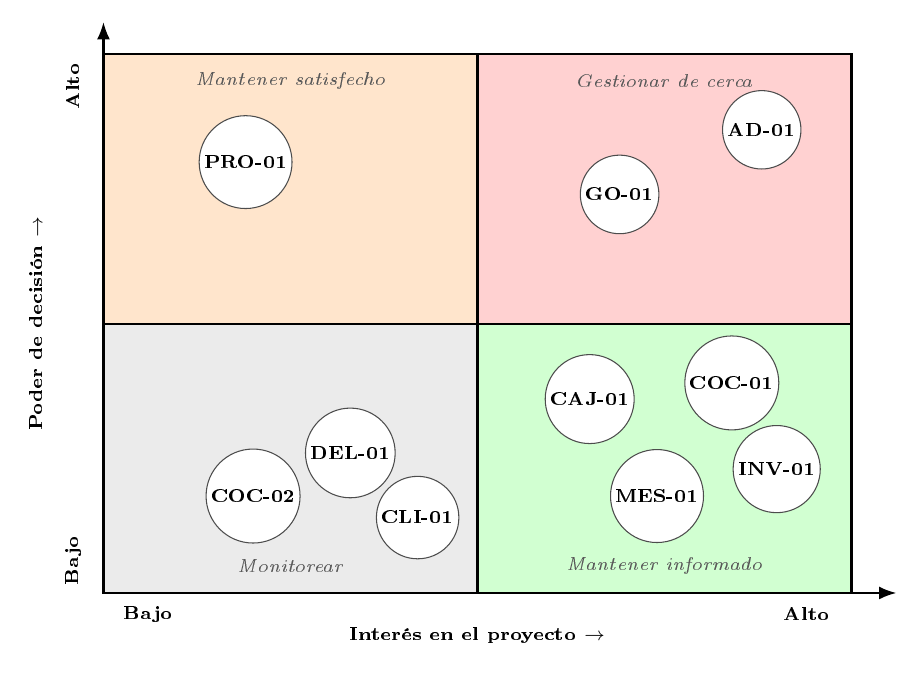
\includegraphics[width=0.88\linewidth]{figuras/poder_interes.png}
\caption{Matriz poder--inter\'es propuesta para El Balcón Restaurant.}
\label{fig:matriz}
\end{figure}

\subsection{Estrategia de participaci\'on por cuadrante}
\begin{itemize}[leftmargin=18pt,itemsep=3pt]
    \item \textbf{Alto poder y alto inter\'es (AD-01, GO-01):} gestionar de cerca. Se les entrevista al inicio y se les presenta el resultado de cada sesi\'on para obtener decisiones y correcciones.
    \item \textbf{Alto poder y bajo inter\'es (PRO-01):} mantener satisfecho. Se le informa solo sobre lo que afecta reposiciones, sin solicitar datos sensibles.
    \item \textbf{Bajo poder y alto inter\'es (COC-01, COC-02, MES-01, CAJ-01, INV-01, DEL-01, CLI-01):} mantener informado. Se les aplica la t\'ecnica que corresponda y se les devuelve un resumen an\'onimo de lo aportado.
    \item \textbf{Bajo poder y bajo inter\'es:} monitorear. No se han asignado roles a este cuadrante en la entrega 1.
\end{itemize}

La estrategia anterior guarda coherencia con las t\'ecnicas planificadas en la secci\'on~7 y con los instrumentos de los ap\'endices: a cada rol se le aplica solo la t\'ecnica que puede responder al tipo de conocimiento que posee \cite{ireb2026}.

\section{Contexto del sistema}
\label{sec:contexto}

\subsection{Límite del sistema y contexto propuesto}
El límite del Sistema de Gestión para Restaurante con IA (SGR-IA) se ubica en la interfaz entre la operación de sala, cocina, caja e inventario de El Balcón Restaurant y las personas que interactúan con ella. La figura~\ref{fig:contexto} presenta las entidades externas y los flujos de información identificados a partir del dominio del negocio y de cuatro entrevistas de campo aplicadas con la guía corregida de 45 preguntas. La cláusula 6.3.3.2 de ISO/IEC/IEEE 29148:2018 dispone identificar a las partes interesadas a lo largo del ciclo de vida y definir una estrategia para elicitar sus necesidades y transformarlas en requisitos \cite{iso29148}; en coherencia con ese criterio, el diagrama distingue las entidades que interactúan con el sistema de los sistemas externos que quedan fuera de alcance, como la facturación electrónica.

\begin{figure}[htbp]
\centering
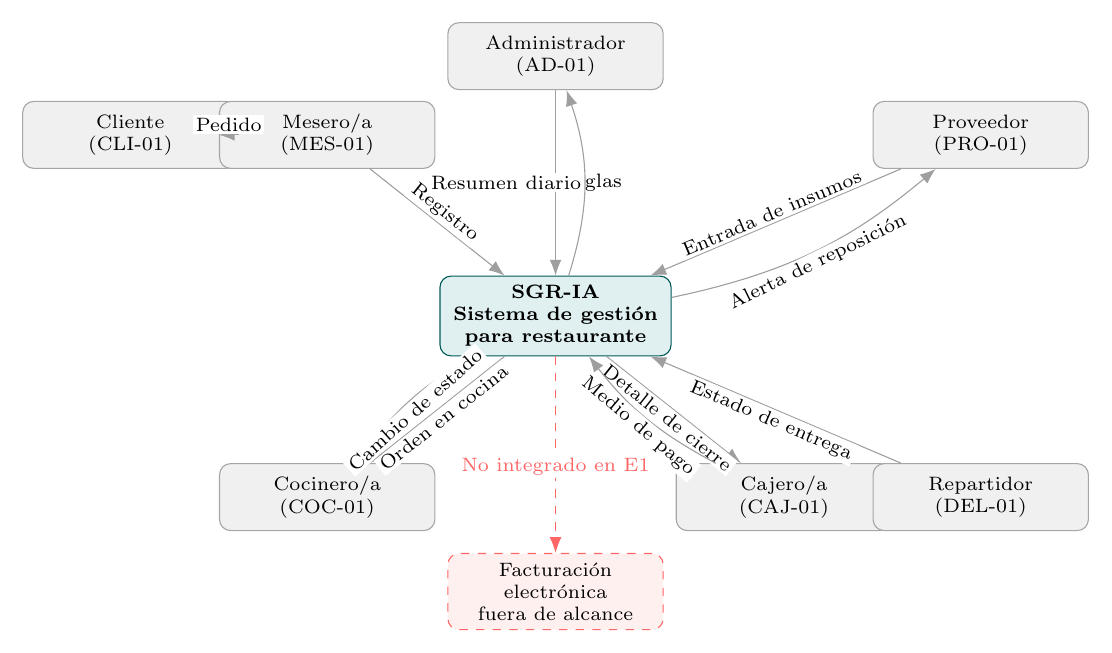
\includegraphics[width=0.90\linewidth]{figuras/contexto.png}
\caption{Contexto del SGR-IA y entidades externas.}
\label{fig:contexto}
\end{figure}

\subsection{Participantes de campo y trato de la información}
Las transcripciones corregidas \texttt{ENTR-01} a \texttt{ENTR-04} son evidencia de campo obtenida por el equipo en El Balcón Restaurant. Usan únicamente códigos de participante y no contienen nombres, cédulas, teléfonos ni correos. Por decisión de custodia, las transcripciones y grabaciones permanecen en carpeta privada `@uteq.edu.ec`; en este documento solo se usan paráfrasis anónimas, sin citas textuales, porque `ENTR-02` no autorizó citar frases literalmente ni depositar sus datos en un repositorio abierto. Los originales firmados de los cuatro formularios de consentimiento se recibieron el 21/11 y se custodian en la carpeta privada `@uteq.edu.ec`; sus nombres, fechas y huellas constan en el manifiesto. La fecha manuscrita de cada formulario no puede leerse con fiabilidad en la copia digital, por lo que no se afirma que el consentimiento haya sido previo a las sesiones. Las fechas informadas son 18/11 (ENTR-01), 19/11 (ENTR-02), 20/11 (ENTR-04) y 21/11 (ENTR-03); las duraciones constan en el manifiesto. Adem\'as de los videos, se recibieron los audios de las cuatro sesiones en \texttt{audio.p.zip}; se conservan en la carpeta privada con los mismos c\'odigos \texttt{ENTR-01} a \texttt{ENTR-04}. Sus duraciones y huellas SHA-256 figuran en el manifiesto como EV-18 a EV-21. El informe no reproduce fragmentos de audio ni datos personales de los participantes.

\begin{table}[htbp]
\centering
\footnotesize
\begin{tabularx}{\linewidth}{|p{1.7cm}|X|p{2.0cm}|p{2.5cm}|}
\hline
\thdr{Código} & \thdr{Rol declarado} & \thdr{Antigüedad} & \thdr{Volumen informado (normal / alto)}\\
\hline
ENTR-01 & Administradora & 1 año 1 mes & 25--30 / 50 personas\\
\hline
ENTR-02 & Cocinera & 2 años & 25 / 35 platos\\
\hline
ENTR-03 & Auxiliar de cocina & 3 años & 45 / 85 pedidos\\
\hline
ENTR-04 & Cajera & 3 años & 60 / 120 pedidos\\
\hline
\end{tabularx}
\caption{Participantes de campo y volúmenes informados por rol.}
\label{tab:participantes}
\end{table}

Los roles de la tabla~\ref{tab:participantes} fueron informados por el equipo
el 21/11; las transcripciones conservan su redacción original y no se han
modificado para ajustarlos.

Las cifras de la tabla~\ref{tab:participantes} no son homogéneas: cada persona mide una unidad distinta (personas, platos o pedidos) en días diferentes. Por ello no se promedian ni se presentan como un dato único de la organización; quedan sujetas a confirmación con el responsable. Las fechas y duraciones reales, tomadas de las grabaciones y de lo informado por el equipo, se registran en el manifiesto; dos de los videos llevan en su título original el nombre del líder, quien realizó y grabó las entrevistas.

\subsection{Ocho perspectivas de análisis del contexto}
La tabla~\ref{tab:perspectivas} actualiza las ocho perspectivas con los hallazgos de campo disponibles. Cuando la información solo proviene de la propuesta inicial se conserva la etiqueta \emph{propuesta}; cuando proviene de las entrevistas se indica el código del participante. Ninguna celda afirma una meta cuantitativa acordada con el responsable, porque esa validación aún no se ha realizado.

\begin{table}[htbp]
\centering
\footnotesize
\begin{tabularx}{\linewidth}{|p{2.5cm}|X|p{2.0cm}|}
\hline
\thdr{Perspectiva} & \thdr{Hallazgo de campo o propuesta} & \thdr{Estado}\\
\hline
Objetivos de negocio & Reducir espera y errores; dolencias: cierre de caja de unas 1--2 h (ENTR-04), conteo de insumos (ENTR-03) y avisos de días sin servicio (ENTR-01). & Parcial\\
\hline
Usuarios y roles & Administradora (ENTR-01), cocinera (ENTR-02), auxiliar de cocina (ENTR-03) y cajera (ENTR-04). Deciden la jefa o el encargado; equipo de 3 a 7 personas. & Campo\\
\hline
Tareas y flujos & Comanda en papel, cocina y caja (ENTR-01/04); domicilio por WhatsApp y moto (ENTR-01/03); cambios comunicados de palabra y no anotados (ENTR-03/04). & Campo\\
\hline
Información y datos & Cuaderno, libreta, pizarra y planilla final; errores por letra poco clara y pedidos modificados sin registro (ENTR-04); stock no se actualiza de inmediato (ENTR-03). & Campo\\
\hline
Funciones del sistema & Registro de pedidos, reservas, inventario, caja y reportes; facturación electrónica permanece fuera del límite (sección~\ref{sec:alcance}). & Propuesta\\
\hline
Comportamiento y estados & Pedido tomado, en cocina, listo y cobrado; domicilio tomado, preparado, en reparto y entregado (ENTR-03/04). Hoy no hay estados informáticos. & Parcial\\
\hline
Calidad y atributos & Errores «pocas veces al mes» (ENTR-01/02/04); la espera y el cobro concentran las molestias; se requiere cuidado con datos de personal y clientes (ENTR-01/03/04). & Campo\\
\hline
Restricciones e interfaces & WhatsApp, efectivo, transferencia y tarjeta, reparto en moto, conectividad y SRI; seis proveedores (ENTR-03); recetas no escritas (ENTR-03/04). & Parcial\\
\hline
\end{tabularx}
\caption{Ocho perspectivas del contexto actualizadas con entrevistas de campo.}
\label{tab:perspectivas}
\end{table}

La tabla~\ref{tab:perspectivas} será revisada con el responsable de la organización para cerrar metas medibles, estados autorizados y prioridades. Las celdas marcadas como \emph{parcial} o \emph{propuesta} no deben interpretarse como acuerdos validados.

\section{Plan de elicitaci\'on}
\label{sec:plan_elicitacion}
\sloppy

Esta secci\'on describe el plan de sesiones de elicitaci\'on complementaria y de validaci\'on con la organizaci\'on. Los hallazgos ya obtenidos de las cuatro entrevistas de campo se presentan en la secci\'on~6; por ello no se repiten aqu\'i el diagrama de contexto ni la tabla de ocho perspectivas. Las fechas de las sesiones propuestas quedan sujetas a la disponibilidad confirmada por El Balcón Restaurant.

\subsection{Definiciones operativas}
Se entiende por \textbf{parte interesada} a la persona o rol con inter\'es leg\'timo en el sistema a lo largo de su ciclo de vida, incluidos quienes influyen en los objetivos y la operaci\'on \cite{iso29148}. El \textbf{l\'imite del sistema} es la frontera entre los procesos que el SGR-IA abarcar\'a --pedidos, cocina, inventario y ventas-- y las entidades externas que quedan fuera, como la facturaci\'on electr\'onica (secci\'on~\ref{sec:alcance}). El \textbf{contexto} es el entorno de uso en el que esas partes interact\'an, representado en la figura~\ref{fig:contexto}. Una \textbf{t\'ecnica de elicitaci\'on} es el procedimiento para obtener conocimiento de una fuente: seg\'un el syllabus IREB \cite{ireb2026}, la entrevista accede al conocimiento expl\'icito que la persona puede relatar y la observaci\'on revela el conocimiento t\'acito que solo aparece al ejecutar la tarea. Estas definiciones delimitan las decisiones de esta entrega y evitan afirmaciones aplicables a cualquier sistema.

\begin{table}[htbp]
\centering
\footnotesize
\begin{tabularx}{\linewidth}{|X|p{2.5cm}|p{2.8cm}|X|}
\hline
\thdr{Parte interesada} & \thdr{Conocimiento} & \thdr{T\'ecnica} & \thdr{Instrumento}\\
\hline
AD-01 (responsable) & Expl\'icito & Entrevista semiestructurada & Guion de entrevista (A)\\
\hline
COC-01, COC-02 (cocina) & T\'acito y expl\'icito & Observaci\'on y taller & Gu\'ias C y A\\
\hline
CAJ-01 (caja) & Expl\'icito & Entrevista y cuestionario & Guion (A) y cuestionario (B)\\
\hline
INV-01 (inventario) & Expl\'icito & Cuestionario estandarizado & Cuestionario (B)\\
\hline
\end{tabularx}
\caption{Correspondencia entre parte interesada, conocimiento, t\'ecnica e instrumento.}
\label{tab:interesado_tecnica}
\end{table}

La tabla~\ref{tab:interesado_tecnica} resume las decisiones para los roles clave; la tabla~\ref{tab:tecnicas} las extiende al resto de las fuentes identificadas.

\subsection{Selecci\'on de t\'ecnicas seg\'un fuente y tipo de conocimiento}
La selecci\'on considera si el conocimiento buscado es expl\'icito --el que la persona puede relatar-- o t\'acito --el que solo aparece al observar la tarea--, seg\'un los fundamentos del syllabus IREB \cite{ireb2026} y de la ingenier\'ia de requisitos \cite{pohl2025}. La tabla~\ref{tab:tecnicas} vincula cada fuente con la t\'ecnica propuesta.

\begin{table}[htbp]
\centering
\footnotesize
\begin{tabularx}{\linewidth}{|p{2.2cm}|p{3.0cm}|p{2.3cm}|X|}
\hline
\thdr{Fuente (c\'odigo)} & \thdr{T\'ecnica} & \thdr{Conocimiento} & \thdr{Justificaci\'on}\\
\hline
AD-01 & Entrevista semiestructurada & Expl\'icito & Permite obtener objetivos, prioridades y criterios de \'exito directamente del responsable.\\
\hline
GO-01 & Taller de modelado de flujos & T\'acito y expl\'icito & Facilita reconstruir el recorrido del pedido con quien coordina turnos.\\
\hline
COC-01 & Observaci\'on + entrevista corta & T\'acito & Revela esperas y reprocesos que no suelen mencionarse en una entrevista.\\
\hline
COC-02 & Observaci\'on an\'onima y preguntas en taller & T\'acito & Registra reprocesos sin exponer a quien ejecuta la tarea.\\
\hline
MES-01 & Observaci\'on en sala & T\'acito & Captura la transmisi\'on verbal del pedido y sus puntos de p\'erdida.\\
\hline
CAJ-01 & Entrevista focalizada & Expl\'icito & Aporta reglas de cierre, medios de pago y formatos de resumen.\\
\hline
INV-01 & Cuestionario & Expl\'icito & Recoge entradas, salidas y frecuencia de conteo de forma estandarizada.\\
\hline
DEL-01 & Cuestionario breve & Expl\'icito & Describe el estado de entrega sin exigir una sesi\'on presencial.\\
\hline
CLI-01 & Cuestionario an\'onimo & Expectativas & Obtiene expectativas de servicio sin exponer datos personales.\\
\hline
PRO-01 & Contacto indirecto por INV-01 & Expl\'icito & Recoge plazos de reposici\'on sin solicitar datos del proveedor.\\
\hline
\end{tabularx}
\caption{T\'ecnicas de elicitaci\'on por fuente y tipo de conocimiento.}
\label{tab:tecnicas}
\end{table}

\subsection{Cronograma de sesiones propuesto}
Las fechas de la tabla~\ref{tab:sesiones} son una propuesta de las semanas 5 y 6 del SPA 2026--2027 y quedan sujetas a la disponibilidad confirmada por El Balcón Restaurant.

\begin{table}[htbp]
\centering
\footnotesize
\begin{tabularx}{\linewidth}{|l|p{1.9cm}|p{2.6cm}|p{2.7cm}|X|}
\hline
\thdr{Sesi\'on} & \thdr{Semana} & \thdr{Participantes} & \thdr{T\'ecnica} & \thdr{Producto esperado}\\
\hline
S1 & 5 & AD-01, GO-01 & Entrevista y taller & Visi\'on y flujo actual acordados.\\
\hline
S2 & 5 & MES-01, COC-01 & Observaci\'on en turno & Notas an\'onimas de tiempos y reprocesos.\\
\hline
S3 & 6 & CAJ-01, INV-01 & Entrevista y cuestionario & Reglas de caja e inventario.\\
\hline
S4 & 6 & DEL-01, CLI-01 & Cuestionario breve & Expectativas de entrega y servicio.\\
\hline
S5 & 6 & AD-01, GO-01 & Validaci\'on & Revisiones al contexto y a las ocho perspectivas.\\
\hline
\end{tabularx}
\caption{Cronograma propuesto de sesiones de elicitaci\'on.}
\label{tab:sesiones}
\end{table}

\subsection{Instrumentos de apoyo}
Se entregan tres instrumentos en los ap\'endices: el guion de entrevista (Ap\'endice~A), el cuestionario (Ap\'endice~B) y la gu\'ia de observaci\'on y taller (Ap\'endice~C). Los tres usan c\'odigos de rol, recogen exclusivamente lo necesario para la elicitaci\'on y explican al participante el tratamiento de sus datos antes de aplicarse, de acuerdo con la LOPDP \cite{lopdp2021}.

\providecommand{\iquest}[1]{¿#1}
\section{Gestión del proyecto}
\sloppy

\subsection{Roles y responsabilidades del equipo}
La organización del trabajo sigue los principios de integración y definición del alcance del PMBOK \cite{pmbok2021}. La tabla~\ref{tab:roles} reparte las responsabilidades verificables de la entrega 1.

\begin{table}[htbp]
\centering
\footnotesize
\begin{tabularx}{\linewidth}{|p{3.4cm}|X|}
\hline
\thdr{Integrante} & \thdr{Responsabilidades en la entrega 1}\\
\hline
Robinson Espinoza Jeanpierre (l\'ider) & Visi\'on, alcance y objetivos; relaci\'on con la organizaci\'on; consentimiento y custodia LOPDP; integraci\'on de \texttt{main.tex}, compilaci\'on y PDF del SGA.\\
\hline
Naranjo Alfonzo Anthony Alexander & Elicitaci\'on y modelado: t\'ecnicas por fuente, instrumentos, contexto y matriz poder--inter\'es en fuentes editables.\\
\hline
S\'anchez Centeno Roselyn Andreina & An\'alisis y calidad documental: partes interesadas, estrategia de participaci\'on, coherencia y trazabilidad, referencias IEEE y revisi\'on del PDF.\\
\hline
\end{tabularx}
\caption{Roles y responsabilidades del equipo.}
\label{tab:roles}
\end{table}

\subsection{Cronograma hasta la semana 17}
La tabla~\ref{tab:cronograma} planifica el trabajo desde la semana 4 hasta la semana 17 del SPA 2026--2027. Las entregas posteriores a la semana 4 se enuncian como plan de proyecto y no como resultados obtenidos en esta entrega.

\begin{table}[htbp]
\centering
\footnotesize
\begin{tabularx}{\linewidth}{|p{1.7cm}|X|p{3.2cm}|}
\hline
\thdr{Semana} & \thdr{Actividad planificada} & \thdr{Producto}\\
\hline
4 & Visi\'on, alcance y bases de la entrega 1 & \texttt{main.tex}, README, ficha y alcance.\\
\hline
5 & Elicitaci\'on con AD-01, GO-01, MES-01 y COC-01 & Notas an\'onimas y contexto validado.\\
\hline
6 & Elicitaci\'on con CAJ-01, INV-01, DEL-01 y CLI-01 & Instrumentos aplicados y perspectivas revisadas.\\
\hline
7 & An\'alisis y especificaci\'on de requisitos & Lista de requisitos y trazabilidad.\\
\hline
8 & Modelado funcional y de datos & Modelos editables exportados.\\
\hline
9 & Validaci\'on de requisitos con la organizaci\'on & Registro de cambios acordados.\\
\hline
10 & Dise\~no de prototipo & Prototipo navegable.\\
\hline
11--12 & Construcci\'on del prototipo y pruebas unitarias & Versiones incrementales.\\
\hline
13 & Pruebas de integraci\'on y usabilidad & Informe de pruebas.\\
\hline
14 & Ajustes seg\'un validaci\'on & Prototipo corregido.\\
\hline
15 & Preparaci\'on de la entrega 2 & Documentaci\'on y fuentes.\\
\hline
16 & Revisi\'on final y ensayo & PDF y repositorio listos.\\
\hline
17 & Cierre del PFC & Entrega final.\\
\hline
\end{tabularx}
\caption{Cronograma del proyecto hasta la semana 17.}
\label{tab:cronograma}
\end{table}

\subsection{Plan de comunicaci\'on con la organizaci\'on}
La tabla~\ref{tab:comunicacion} precisa con qui\'en se comunica el equipo, en qu\'e momento del plan, por qu\'e canal y con qu\'e frecuencia. Las sesiones S1 a S5 corresponden al cronograma propuesto en la secci\'on~7; las fechas quedan sujetas a la disponibilidad confirmada por El Balcón Restaurant.

\begin{table}[htbp]
\centering
\footnotesize
\begin{tabularx}{\linewidth}{|p{2.4cm}|p{2.6cm}|X|p{2.7cm}|}
\hline
\thdr{Con qui\'en} & \thdr{Cu\'ando} & \thdr{Canal} & \thdr{Frecuencia}\\
\hline
AD-01 & S1 y S5 & Correo institucional \texttt{@uteq.edu.ec} y mensajer\'ia acordada & Una solicitud de agenda por sesi\'on y una validaci\'on formal al cierre de la entrega 1.\\
\hline
GO-01, MES-01, COC-01, COC-02 & S1 y S2 & Coordinaci\'on previa por AD-01; instrumentos impresos o digitales en la sesi\'on & Una convocatoria por sesi\'on y un resumen an\'onimo posterior.\\
\hline
CAJ-01, INV-01, DEL-01 & S3 & Correo institucional y cuestionario estandarizado & Una convocatoria y un recordatorio antes de la sesi\'on.\\
\hline
CLI-01, PRO-01 & S4 & Cuestionario an\'onimo distribuido por AD-01 & Una aplicaci\'on en la semana 6.\\
\hline
Equipo ISR-401 & Despu\'es de cada sesi\'on y al cierre & \texttt{evidencias/REGISTRO\_CONTACTO.md} y registro privado en el manifiesto & Un asiento por contacto y una revisi\'on final antes de la entrega.\\
\hline
\end{tabularx}
\caption{Plan de comunicaci\'on con la organizaci\'on y el equipo.}
\label{tab:comunicacion}
\end{table}

El l\'ider concentra las solicitudes y devuelve los acuerdos; los dem\'as integrantes no contactan a la organizaci\'on por separado sin coordinaci\'on. No se usan correos personales de participantes y cada contacto se anota en \texttt{evidencias/REGISTRO\_CONTACTO.md}, cuyo respaldo privado se registra en el manifiesto con SHA-256.

\subsection{Registro de riesgos}
La tabla~\ref{tab:riesgos} recoge riesgos espec\'ificos de la organizaci\'on y del contexto acad\'emico, con mitigaciones verificables.

\begin{table}[htbp]
\centering
\footnotesize
\begin{tabularx}{\linewidth}{|l|X|p{1.9cm}|X|}
\hline
\thdr{ID} & \thdr{Riesgo} & \thdr{Impacto} & \thdr{Mitigaci\'on}\\
\hline
R1 & Disponibilidad limitada de AD-01 por atenci\'on del local & Alto & Agendar con antelaci\'on y preparar res\'umenes breves para validaci\'on.\\
\hline
R2 & Ruido e interrupciones en sala durante la observaci\'on & Medio & Observar en turnos de baja demanda y registrar solo c\'odigos de rol.\\
\hline
R3 & Rotaci\'on de personal antes de la validaci\'on & Medio & Documentar el rol, no la persona, y repetir la sesi\'on cr\'itica con el reemplazo.\\
\hline
R4 & Sensibilidad de datos de clientes y proveedores & Alto & Excluir identificadores personales y aplicar anonimizaci\'on desde el instrumento.\\
\hline
R5 & Conectividad insuficiente en el local & Medio & Dise\~nar instrumentos impresos y probar la soluci\'on con datos locales.\\
\hline
R6 & Dependencia de una sola fuente para el flujo de pedidos & Medio & Contrastar entrevista, observaci\'on y cuestionario.\\
\hline
R7 & Carga acad\'emica concurrente en semana 16 & Medio & Cerrar fuentes y compilaci\'on antes de la semana 15.\\
\hline
\end{tabularx}
\caption{Registro de riesgos de la entrega 1.}
\label{tab:riesgos}
\end{table}

\subsection{\'Etica, consentimiento y custodia}
El tratamiento de datos se rige por la LOPDP \cite{lopdp2021} y por el C\'odigo de \'Etica de la ACM \cite{acm2018}. Se emplean c\'odigos de rol, se excluyen c\'edulas, tel\'efonos, correos personales, audios y firmas del repositorio p\'ublico, y los cuatro originales firmados se recibieron como fotografías el 21/11, se custodian en la carpeta institucional privada \texttt{@uteq.edu.ec} y se registran como EV-14 a EV-17 con el formato \texttt{AAAA-MM-DD\_Rol\_Codigo\_Consentimiento}, sin nombres personales. La fecha manuscrita de cada formulario no puede leerse con fiabilidad en la copia digital, por lo que no se afirma que el consentimiento haya sido previo a las sesiones. El modelo en blanco se entrega en \texttt{evidencias/MODELO\_CONSENTIMIENTO\_INFORMADO\_SGR1.tex}; el repositorio incluye el modelo en blanco, sin datos personales, y remite al manifiesto para el registro de los originales firmados. La carta de aceptaci\'on y el registro de primer contacto siguen la misma regla. Los audios y videos de las cuatro entrevistas, las transcripciones y las actas permanecen en la carpeta privada; el repositorio solo publica sus nombres de archivo, fechas, duraciones y huellas SHA-256. Este procedimiento evita exponer datos personales y permite al docente verificar la custodia sin acceder a los originales desde un repositorio abierto.

\subsection{Verificaci\'on de la evidencia de campo}
El manifiesto \texttt{evidencias/MANIFIESTO.md} registra 21 evidencias privadas (EV-01 a EV-21) con nombre de archivo, fecha, duraci\'on cuando aplica y huella SHA-256. Las evidencias EV-01 y EV-02 documentan la aceptaci\'on de la organizaci\'on y el primer contacto; EV-03 a EV-06 son las transcripciones corregidas; EV-07 a EV-09 son adendums por \'items omitidos en la transcripci\'on; EV-10 a EV-13 son los videos; EV-14 a EV-17 son los formularios de consentimiento firmados; y EV-18 a EV-21 son los audios. Ning\'un archivo identificable se sube al repositorio.

La verificaci\'on se apoya en tres criterios: (i) que el c\'odigo \texttt{ENTR-xx} sea el mismo en transcripci\'on, video, audio y formulario; (ii) que la fecha informada por el equipo y la duraci\'on del archivo coincidan con el registro; y (iii) que la huella SHA-256 permita comprobar que el archivo privado no cambi\'o. Cuando el nombre original de una grabaci\'on discrepaba con la fecha informada, se conserv\'o la fecha informada y se dej\'o constancia de la discrepancia en \texttt{INTEGRIDAD.md}. Este procedimiento no subsana la falta de consentimiento previo verificable; por eso el informe usa \'unicamente par\'afrasis an\'onimas y no publica citas textuales de las participantes.


% ==============================================================================
% SECCIONES 6 Y 7: CONTEXTO Y PLAN DE ELICITACION (Naranjo Alfonzo Anthony Alexander)
% ==============================================================================

\newpage
\appendix
\providecommand{\iquest}[1]{¿#1}
\section{Guion de entrevista semiestructurada}
\sloppy

\textbf{C\'odigo del instrumento:} INS-ENT-01. \textbf{Duraci\'on estimada:} 35 a 50 minutos.
\textbf{Dirigido a:} personal de atenci\'on, cocina, caja e inventario de
El Balcón Restaurant. \textbf{Registro:} notas an\'onimas con c\'odigo de rol; sin
grabaci\'on salvo autorizaci\'on expresa.

\textbf{Origen del instrumento.} Este guion reproduce, sin respuestas de ejemplo,
las 45 preguntas de \texttt{guia\_entrevista\_restaurante1\_corregida.pdf},
documento UTEQ empleado en la aplicaci\'on de campo. La versi\'on corregida se
incorpora como instrumento en blanco; las versiones con respuestas redactadas
(`003.pdf`, `004.pdf` y `005.pdf') se usaron solo como apoyo para redactar el
guion y \emph{no} como resultados de la entrevista.

\subsection*{Apertura y consideraciones \'eticas}
Se lee al participante:

\begin{quote}
\small
``Esta entrevista se realiza con el prop\'osito de levantar informaci\'on sobre
la operaci\'on diaria del restaurante: las actividades que realiza el personal,
la forma en que se atienden y registran los pedidos, se controla el inventario,
se gestionan las compras, el personal y la informaci\'on administrativa. La
informaci\'on recolectada permitir\'a describir la situaci\'on actual del
establecimiento y servir\'a \'unicamente como insumo para un trabajo acad\'emico.
La entrevista no eval\'ua el desempe\~no de la persona entrevistada ni busca
proponer soluciones en esta etapa. La participaci\'on es voluntaria; no se
solicitan nombre, c\'edula, tel\'efono ni correo. Puede interrumpir la entrevista
o abstenerse de responder sin justificaci\'on. \iquest{Autoriza el uso an\'onimo
de sus respuestas para este proyecto?}''
\end{quote}

Si se autoriza grabaci\'on, se anota el c\'odigo del participante, la fecha, la
hora de inicio y de finalizaci\'on y la duraci\'on real. El original firmado y la
grabaci\'on se custodian en carpeta privada \texttt{@uteq.edu.ec}.

\subsection*{1. Apertura y perfil del cargo}
\begin{enumerate}[leftmargin=18pt,itemsep=0pt]
    \item \iquest{Cu\'al es su cargo y cu\'anto tiempo lleva en el restaurante?}
    \item \iquest{Cu\'ales son sus responsabilidades en un d\'ia normal y con qu\'e \'areas interact\'ua m\'as?}
    \item \iquest{Qu\'e medio o forma utiliza para registrar actualmente las actividades de su trabajo?}
\end{enumerate}

\subsection*{2. Gesti\'on de pedidos y ventas}
\begin{enumerate}[leftmargin=18pt,itemsep=0pt,resume]
    \item \iquest{C\'omo se atiende un pedido, desde que llega el cliente hasta que paga?}
    \item \iquest{C\'omo se registra cada pedido y cu\'antos se atienden en un d\'ia normal y en uno de mayor movimiento?} D\'ia normal: \rule{1.6cm}{0.4pt}; d\'ia de mayor movimiento: \rule{1.6cm}{0.4pt}.
    \item \iquest{Qu\'e es lo que m\'as se le dificulta cuando hay mucha demanda?}
    \item \iquest{Con qu\'e frecuencia ocurren errores en los pedidos?} a) Nunca; b) Pocas veces al mes; c) Varias veces por semana; d) Todos los d\'ias. \iquest{Por qu\'e cree que ocurren?}
    \item \iquest{C\'omo se realiza el cobro y la facturaci\'on?} \iquest{Qu\'e medios de pago se aceptan y qu\'e inconvenientes ha tenido al cobrar, dividir cuentas o facturar?}
\end{enumerate}

\subsection*{3. Gesti\'on de delivery y entrega a domicilio}
\begin{enumerate}[leftmargin=18pt,itemsep=0pt,resume]
    \item \iquest{El restaurante ofrece servicio de entrega a domicilio?} \iquest{C\'omo se solicita y con qu\'e frecuencia se utiliza?}
    \item \iquest{C\'omo se recibe y registra un pedido para entrega a domicilio?}
    \item \iquest{C\'omo se organiza la preparaci\'on y el despacho de los pedidos a domicilio para que lleguen a tiempo?}
    \item \iquest{Qu\'e medio de transporte o repartidores se utilizan y c\'omo se asigna cada entrega?}
    \item \iquest{Qu\'e problemas ocurren con m\'as frecuencia en las entregas a domicilio (demoras, pedidos incompletos, direcciones, cobros) y c\'omo se resuelven?}
\end{enumerate}

\subsection*{4. Gesti\'on de reservas y atenci\'on al cliente}
\begin{enumerate}[leftmargin=18pt,itemsep=0pt,resume]
    \item \iquest{C\'omo se registra y confirma una reserva?} \iquest{C\'omo se decide qu\'e mesa se asigna a cada cliente o grupo?}
    \item \iquest{Con qu\'e frecuencia hay problemas con mesas o reservas (cruces, esperas, cancelaciones)?} a) Nunca; b) Rara vez; c) Con frecuencia; d) Casi siempre. \iquest{Por qu\'e cree que ocurren?}
    \item \iquest{C\'omo se atienden las solicitudes especiales de los clientes (alergias, celebraciones, preferencias)?}
    \item \iquest{Qu\'e es lo que m\'as reclaman los clientes?} a) Tiempo de espera; b) Errores en el pedido; c) Trato del personal; d) Precios o cobros; e) Otro. \iquest{Por qu\'e cree que ocurre?}
\end{enumerate}

\subsection*{5. Gesti\'on de cocina y preparaci\'on de alimentos}
\begin{enumerate}[leftmargin=18pt,itemsep=0pt,resume]
    \item \iquest{C\'omo llega la comanda a la cocina y c\'omo se decide el orden en que se preparan los pedidos?}
    \item \iquest{C\'omo se comunican cocina y meseros cuando un pedido est\'a listo o cambia?}
    \item \iquest{Con qu\'e frecuencia se retrasan los platos?} a) Nunca; b) Algunas veces; c) Frecuentemente; d) Casi siempre. \iquest{Cu\'al es la causa principal?}
    \item \iquest{C\'omo se controla que los platos se preparen con la misma receta y porci\'on?} \iquest{Qu\'e hacen cuando falta un ingrediente en pleno servicio?}
\end{enumerate}

\subsection*{6. Gesti\'on de inventario}
\begin{enumerate}[leftmargin=18pt,itemsep=0pt,resume]
    \item \iquest{C\'omo se controlan los productos e insumos y c\'omo se registran las entradas y salidas?}
    \item \iquest{Cada cu\'anto se revisa el inventario?} a) Diariamente; b) Semanalmente; c) Mensualmente; d) Solo cuando falta algo. \iquest{Por qu\'e con esa frecuencia?}
    \item \iquest{C\'omo y d\'onde se almacenan los insumos, sobre todo los perecederos?}
    \item \iquest{Con qu\'e frecuencia hay productos vencidos, da\~nados o desperdiciados?} \iquest{C\'omo se decide cu\'ando y cu\'anto reponer de cada producto?}
\end{enumerate}

\subsection*{7. Gesti\'on de compras y proveedores}
\begin{enumerate}[leftmargin=18pt,itemsep=0pt,resume]
    \item \iquest{C\'omo se solicitan los productos a los proveedores y qui\'en decide qu\'e se compra y en qu\'e cantidades?}
    \item \iquest{Con cu\'antos proveedores trabajan y c\'omo se verifica que lo recibido coincida con lo pedido y lo facturado?}
    \item \iquest{Con qu\'e frecuencia hay problemas con proveedores (retrasos, faltantes, calidad)?} a) Nunca; b) Rara vez; c) Con frecuencia; d) Casi siempre. \iquest{Cu\'ales son los problemas m\'as comunes y por qu\'e cree que ocurren?}
    \item \iquest{C\'omo se registran las compras y los pagos a proveedores?} \iquest{C\'omo se elige entre proveedores o se comparan precios?}
\end{enumerate}

\subsection*{8. Gesti\'on del personal}
\begin{enumerate}[leftmargin=18pt,itemsep=0pt,resume]
    \item \iquest{Cu\'antas personas trabajan en el restaurante y en qu\'e \'areas?} Total: \rule{1.5cm}{0.4pt}; \'areas: \rule{3cm}{0.4pt}.
    \item \iquest{C\'omo se asignan las tareas a cada empleado y c\'omo se organizan los turnos?}
    \item \iquest{Con qu\'e frecuencia hay ausencias o cambios de \'ultimo minuto?} a) Nunca; b) Rara vez; c) Con frecuencia; d) Casi siempre. \iquest{Por qu\'e cree que ocurre y qu\'e se hace cuando pasa?}
    \item \iquest{C\'omo se coordinan las actividades entre cocina, meseros y caja?} \iquest{C\'omo se supervisa o eval\'ua el desempe\~no del personal?}
\end{enumerate}

\subsection*{9. Gesti\'on administrativa y reportes}
\begin{enumerate}[leftmargin=18pt,itemsep=0pt,resume]
    \item \iquest{C\'omo se registran los ingresos y gastos?}
    \item \iquest{Qu\'e informes elabora o recibe actualmente?} \iquest{Cada cu\'anto y qui\'en los usa?}
    \item \iquest{C\'omo analiza qu\'e productos se venden m\'as o menos?} \iquest{Qu\'e tan f\'acil es obtener la informaci\'on que necesita para decidir?}
\end{enumerate}

\subsection*{10. Dificultades del trabajo diario}
\begin{enumerate}[leftmargin=18pt,itemsep=0pt,resume]
    \item \iquest{Qu\'e tareas de su trabajo le consumen m\'as tiempo o esfuerzo?}
    \item \iquest{Qu\'e informaci\'on del restaurante es m\'as dif\'icil de obtener o mantener actualizada?}
    \item \iquest{Qu\'e ocurre cuando la persona que conoce un proceso no est\'a presente?}
\end{enumerate}

\subsection*{11. Conocimiento y expectativas sobre inteligencia artificial}
\begin{enumerate}[leftmargin=18pt,itemsep=0pt,resume]
    \item \iquest{Qu\'e entiende usted por inteligencia artificial y qu\'e tanto conoce sobre ella?} a) Nada; b) He escuchado el t\'ermino; c) Entiendo lo b\'asico; d) La uso con frecuencia.
    \item \iquest{Ha usado alguna herramienta con inteligencia artificial, en el trabajo o en su vida personal?} \iquest{Cu\'al y c\'omo fue su experiencia?}
    \item \iquest{Qu\'e opina de que un restaurante use inteligencia artificial en su operaci\'on y qu\'e tanto confiar\'ia en su uso?} \iquest{Por qu\'e?}
    \item \iquest{Qu\'e es lo que m\'as le preocupar\'ia sobre el uso de la inteligencia artificial en el trabajo?} a) Que cometa errores; b) Perder el control de las decisiones; c) Que sea dif\'icil de aprender; d) La seguridad de los datos; e) Que reemplace funciones del personal; f) Nada me preocupa; g) Otro. \iquest{Por qu\'e eligi\'o esa opci\'on?}
    \item \iquest{Qu\'e informaci\'on del restaurante considera que deber\'ia mantenerse bajo control humano y no ser manejada por inteligencia artificial?} \iquest{Por qu\'e?}
\end{enumerate}

\subsection*{12. Cierre}
\begin{enumerate}[leftmargin=18pt,itemsep=0pt,resume]
    \item \iquest{Hay alg\'un proceso o problema importante del que no hayamos hablado o algo que desee agregar?}
\end{enumerate}

\noindent\textbf{Observaciones del entrevistador:}\\[0.2cm]
\rule{\linewidth}{0.4pt}\\[0.6cm]
\rule{\linewidth}{0.4pt}

\providecommand{\iquest}[1]{¿#1}
\section{Cuestionario an\'onimo}

\textbf{C\'odigo del instrumento:} INS-CUE-01. \textbf{Dirigido a:} INV-01, DEL-01, CLI-01.
\textbf{Aplicaci\'on:} individual, 5 a 8 minutos. No se solicita nombre, c\'edula, tel\'efono ni correo. El participante solo marca un c\'odigo de rol asignado por el equipo.

\subsection*{Escala}
Para los \'itemos 1 a 8 se usa la escala: 1 = Totalmente en desacuerdo; 2 = En desacuerdo; 3 = Neutral; 4 = De acuerdo; 5 = Totalmente de acuerdo.

\begin{enumerate}[leftmargin=18pt,itemsep=0pt]
    \item El registro actual de pedidos permite saber su estado sin preguntar a otra persona. \quad 1~~2~~3~~4~~5
    \item Los datos que apunto en papel se transcriben despu\'es sin dificultad. \quad 1~~2~~3~~4~~5
    \item Conozco qu\'e insumos cr\'iticos pueden agotarse en el turno. \quad 1~~2~~3~~4~~5
    \item La reposici\'on de insumos se decide con informaci\'on suficiente. \quad 1~~2~~3~~4~~5
    \item Recibo la informaci\'on del pedido con el detalle necesario para mi tarea. \quad 1~~2~~3~~4~~5
    \item El estado de una entrega a domicilio puede consultarse sin llamar por tel\'efono. \quad 1~~2~~3~~4~~5
    \item Un resumen de ventas me resultar\'ia \'util antes del cierre de caja. \quad 1~~2~~3~~4~~5
    \item Me sentir\'ia c\'omodo confirmando una sugerencia autom\'atica de reposici\'on. \quad 1~~2~~3~~4~~5
\end{enumerate}

\subsection*{Preguntas abiertas}
\begin{enumerate}[leftmargin=18pt,itemsep=0pt,start=9]
    \item \iquest{Qu\'e dato se le pide con m\'as frecuencia y no est\'a disponible?}
    \item \iquest{Qu\'e cambio en el proceso de pedido o entrega tendr\'ia mayor impacto?}
    \item \iquest{Qu\'e precauci\'on debe tomar el sistema para no sustituir el criterio humano?}
\end{enumerate}

\subsection*{Registro del aplicador}
C\'odigo de rol del participante: \rule{3cm}{0.4pt}\quad Fecha: \rule{2.5cm}{0.4pt}\quad Duración: \rule{2cm}{0.4pt}.
Se advierte que las respuestas se usar\'an solo para la elicitaci\'on de requisitos y que no se publicar\'an comentarios que permitan identificar a la persona.

\providecommand{\iquest}[1]{¿#1}
\section{Gu\'ia de observaci\'on y taller}

\textbf{C\'odigo del instrumento:} INS-OBS-01. \textbf{Dirigido a:} MES-01, COC-01 y al grupo GO-01.
\textbf{Duración estimada:} 45 minutos de observaci\'on y 60 minutos de taller. Se aplica en el local con autorizaci\'on previa del responsable.

\subsection*{Ficha de sesi\'on}
Fecha: \rule{2.8cm}{0.4pt}\quad Turno: \rule{2.2cm}{0.4pt}\quad \'Area observada: \rule{3cm}{0.4pt}\quad
Observador: \rule{3cm}{0.4pt}\quad C\'odigos de roles presentes: \rule{4cm}{0.4pt}.

\subsection*{Lista de observaci\'on}
Para cada \'item se registra S\'i, No o No observado y una nota breve sin nombres propios.

\begin{enumerate}[leftmargin=18pt,itemsep=1pt]
    \item El pedido se dice en voz alta y se repite para confirmación.
    \item Existe un soporte f\'isico o digital donde se anota el pedido.
    \item La cocina recibe los pedidos en el mismo orden en que llegaron.
    \item Se corrige alg\'un pedido por falta de detalle o por duplicidad.
    \item Se consulta el inventario antes de usar un insumo cr\'itico.
    \item Se registra la salida de insumos en el momento del uso.
    \item El cajero recibe el detalle de lo consumido antes de cerrar.
    \item Se genera un resumen de ventas sin transcripci\'on adicional.
    \item Una sugerencia autom\'atica, si existiera, requerir\'ia confirmación humana.
    \item Se identifica al menos un momento de espera atribuible a la comunicaci\'on.
\end{enumerate}

\subsection*{Din\'amica del taller}
\begin{enumerate}[leftmargin=18pt,itemsep=0pt]
    \item \textbf{Contexto (10 min):} el responsable describe el objetivo del taller y se confirma el uso an\'onimo de lo registrado.
    \item \textbf{Recorrido del pedido (25 min):} en una hoja por turnos se dibuja cada paso, qui\'en lo ejecuta y qu\'e informaci\'on entrega.
    \item \textbf{Puntos de control (15 min):} se marcan con una cruz los pasos donde se detectan errores y con una estrella los que requieren decisi\'on humana.
    \item \textbf{Priorizaci\'on (10 min):} cada participante dispone de tres votos para señalar los puntos cr\'iticos.
\end{enumerate}

\subsection*{Cierre y custodia}
El facilitador lee en voz alta los acuerdos, los códigos de rol y la fecha. El original de las notas se guarda en la carpeta institucional privada \texttt{@uteq.edu.ec}; en el repositorio p\'ublico solo se registra su huella SHA-256 en \texttt{evidencias/MANIFIESTO.md}.

\newpage
\printbibliography[title={Referencias}]

\end{document}

